% fig3_enclosure_perimeter.tex — Figure 4 (column width)
% The Constitutional Enclosure perimeter: three attack vectors rejected by
% the compiler; the only well-typed path is Verdict::new.
% Regenerated 2026-09-15 (COMSI-2026-04-0112 R1), monochrome.
% v2: attacks from west/east/north; boundary label clear of all arrows
% (VLM visual inspection round).
\documentclass[border=2pt]{standalone}
\usepackage{tikz}
\usetikzlibrary{arrows.meta,positioning,fit,calc,shapes.misc}
\usepackage{amssymb}
\begin{document}
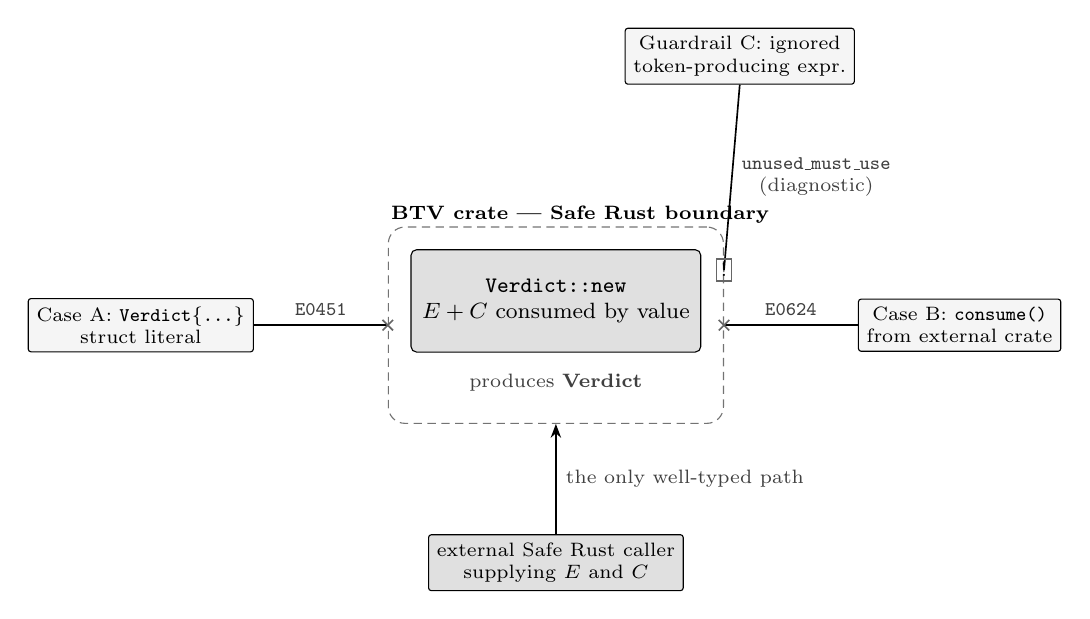
\begin{tikzpicture}[
  font=\footnotesize,
  core/.style={draw, rounded corners=2pt, align=center, inner sep=4pt,
    fill=black!12, minimum height=13mm},
  att/.style={draw, rounded corners=1pt, align=center, inner sep=3pt,
    fill=black!04, font=\scriptsize},
  arr/.style={-{Stealth[length=5pt]}, semithick},
  blk/.style={semithick},
  note/.style={align=center, font=\scriptsize, text=black!75}
]

% ── The perimeter ─────────────────────────────────────────────────────────
\node[core] (vnew) at (0,0)
  {\textbf{\texttt{Verdict::new}}\\ $E + C$ consumed by value};
\node[note, below=1.5mm of vnew] (prod) {produces \textbf{Verdict}};
\node[draw=black!55, rounded corners=6pt, densely dashed,
  fit=(vnew)(prod), inner sep=8pt] (perim) {};
\node[font=\scriptsize\bfseries, anchor=south west, inner sep=1pt]
  at (perim.north west) {BTV crate --- Safe Rust boundary};

% ── Attack vector A (from the west): struct literal ──────────────────────
\node[att, left=17mm of perim.west, anchor=east] (a1)
  {Case A: \texttt{Verdict\{...\}}\\ struct literal};
\draw[blk] (a1.east) -- (perim.west)
  node[midway, above, note] {\texttt{E0451}};
\node[draw=black!60, cross out, semithick, inner sep=1.6pt] at (perim.west) {};

% ── Attack vector B (from the east): external consume() ──────────────────
\node[att, right=17mm of perim.east, anchor=west] (a2)
  {Case B: \texttt{consume()}\\ from external crate};
\draw[blk] (a2.west) -- (perim.east)
  node[midway, above, note] {\texttt{E0624}};
\node[draw=black!60, cross out, semithick, inner sep=1.6pt] at (perim.east) {};

% ── Guardrail C (from the north-east): ignored token-producing expr. ─────
% Not a hard rejection like Cases A/B — matches the proof text's own
% "Guardrail C" framing: the diagnostic catches the plain-ignore case,
% while let _ = expr/drop/mem::forget remain possible (closure instead
% comes from the encapsulation axiom, per the adjacent proof).
\node[att, above right=18mm and 2mm of perim.north east, anchor=south] (a3)
  {Guardrail C: ignored\\ token-producing expr.};
\draw[blk] (a3.south) -- ($(perim.east)+(0,7mm)$)
  node[midway, right, note] {\texttt{unused\_must\_use}\\ (diagnostic)};
\node[draw=black!60, semithick, inner sep=1.6pt]
  at ($(perim.east)+(0,7mm)$) {\scriptsize !};

% ── The only authorized entry ─────────────────────────────────────────────
\node[att, below=14mm of perim.south, fill=black!12] (gate)
  {external Safe Rust caller\\ supplying $E$ and $C$};
\draw[arr] (gate.north) -- (perim.south)
  node[midway, right, note] {the only well-typed path};

\end{tikzpicture}
\end{document}
